\section{Ablation and NYUv2 Figures}
Nash-MTL's per-step coefficients varied substantially across batches in all three runs. This
observation is descriptive only: the present logs do not distinguish solver variation from an
intrinsic property of the method on this benchmark.

\begin{figure*}[t]
\centering
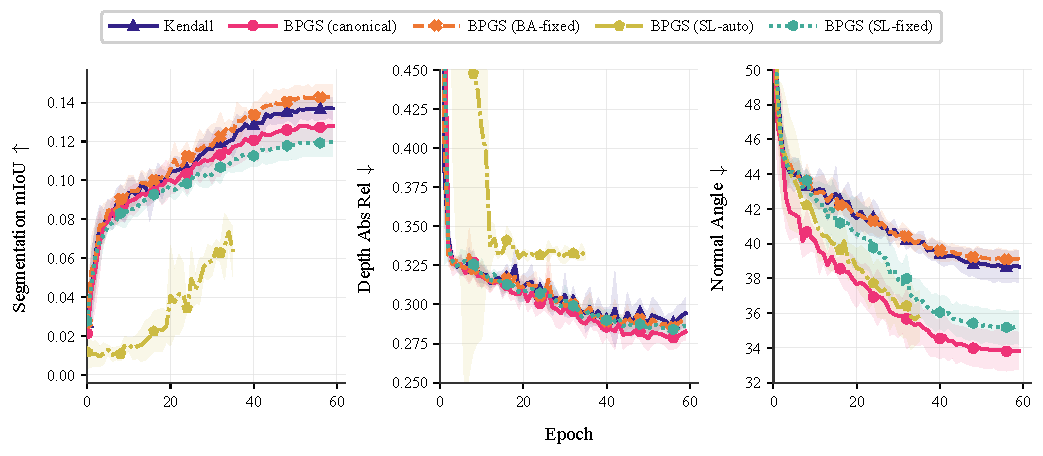
\includegraphics[width=\textwidth]{data/ablation/figures/pdf/ablation_per_task_val_curves.pdf}
\caption{NYUv2 ablation validation curves by task. The stateless auto-calibrated variant fails on segmentation and remains weak on depth, while the batch-aware variants maintain stronger trajectories throughout training.}
\label{fig:appendix_ablation_val_curves}
\end{figure*}

\begin{figure*}[t]
\centering
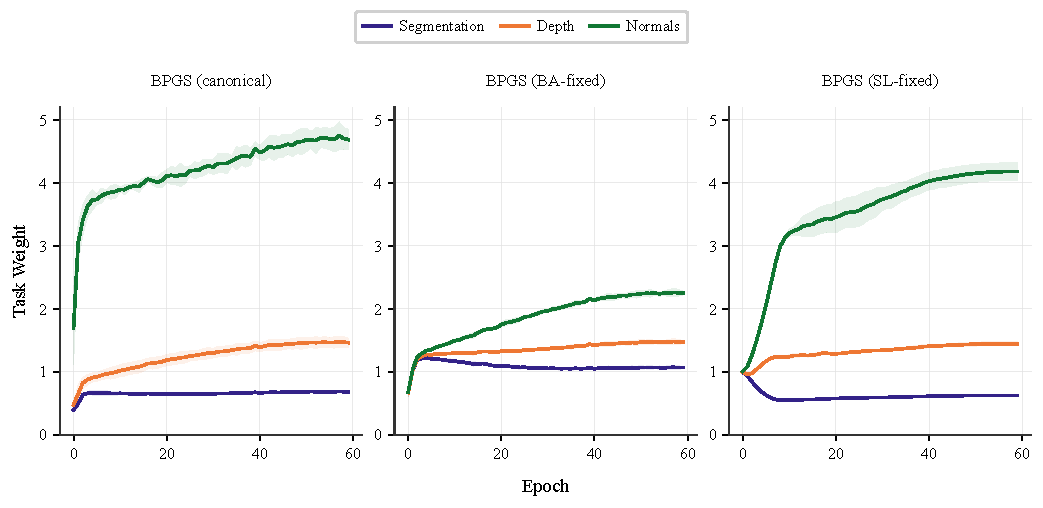
\includegraphics[width=\textwidth]{data/ablation/figures/pdf/ablation_weight_dynamics.pdf}
\caption{Task-weight dynamics for representative stable BPGS variants on the NYUv2 ablation. The batch-aware variants keep task weights in distinct but controlled regimes, whereas the stateless fixed variant shows a different long-run allocation pattern, especially for the surface-normal task.}
\label{fig:appendix_ablation_weights}
\end{figure*}

\begin{figure*}[t]
\centering
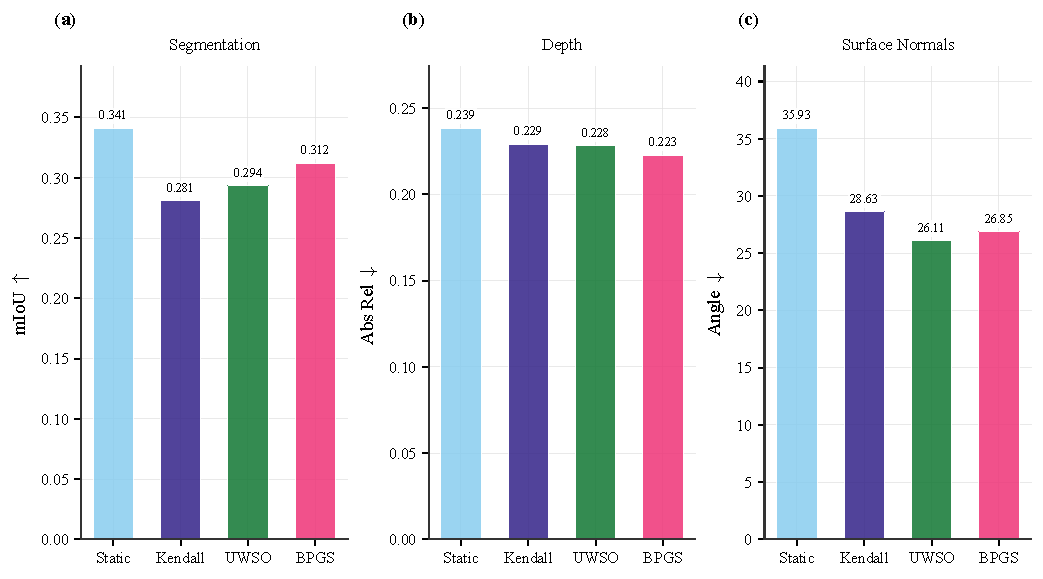
\includegraphics[width=\textwidth]{data/nyuv2/figures/pdf/nyuv2_performance_comparison.pdf}
\caption{NYUv2 per-task performance comparison. The figure makes the trade-off pattern visually explicit: Static is strongest on segmentation, UWSO is strongest on surface normals, and BPGS is strongest on both depth metrics.}
\label{fig:appendix_nyuv2_bars}
\end{figure*}

\begin{figure*}[t]
\centering
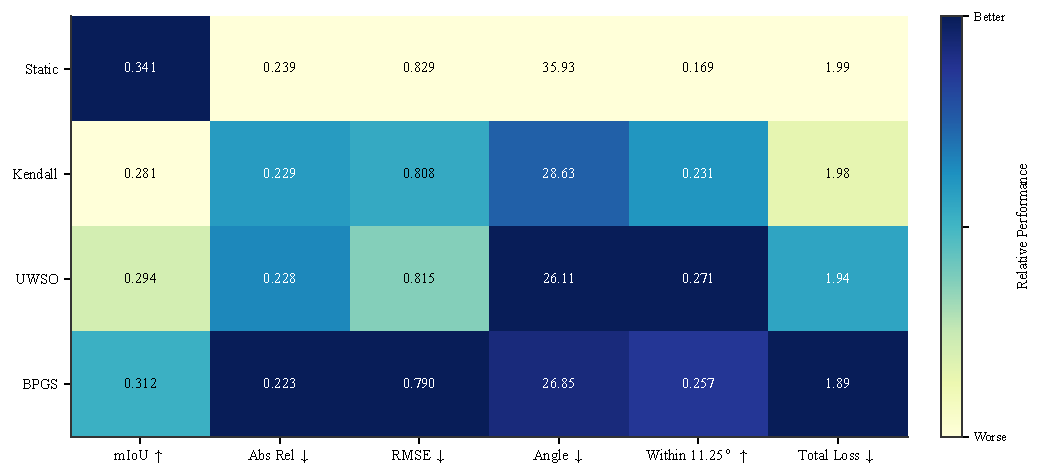
\includegraphics[width=\textwidth]{data/nyuv2/figures/pdf/nyuv2_performance_heatmap.pdf}
\caption{NYUv2 performance heatmap across reported metrics. Darker cells indicate stronger relative performance after accounting for metric direction. BPGS concentrates its gains on depth and total loss, while Static and UWSO remain stronger on some other tasks.}
\label{fig:appendix_nyuv2_heatmap}
\end{figure*}

\begin{figure*}[t]
\centering
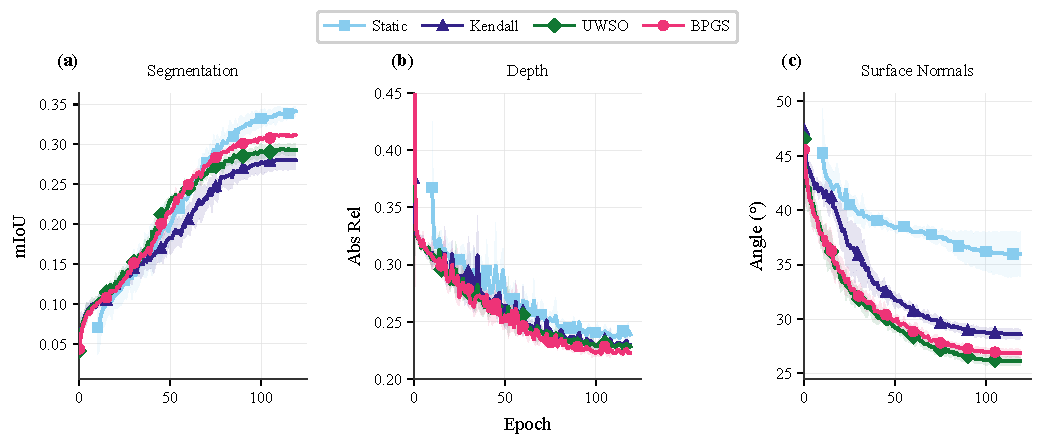
\includegraphics[width=\textwidth]{data/nyuv2/figures/pdf/nyuv2_task_training_curves.pdf}
\caption{NYUv2 validation training curves by task. BPGS tracks the strongest depth trajectory and remains competitive on segmentation and surface normals over the full 120-epoch budget.}
\label{fig:appendix_nyuv2_curves}
\end{figure*}

\begin{figure}[t]
\centering
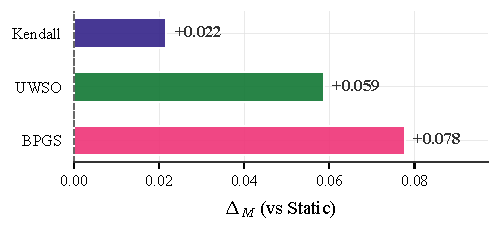
\includegraphics[width=\columnwidth]{data/nyuv2/figures/pdf/nyuv2_delta_m_comparison.pdf}
\caption{NYUv2 $\Delta_M$ comparison against the Static baseline. BPGS attains the strongest aggregate improvement among the adaptive methods evaluated in the main benchmark.}
\label{fig:appendix_nyuv2_delta}
\end{figure}
